\chapter{Test and Evaluation}
\label{ch:evaluation}
The last chapter discussed implementation details for the \textit{"Collector-Platform"} introduced in \autoref{ch:architecture}.
For its realization, Java 8 as programming language head been chosen in combination with the Spring Boot framework which allowed
the rapid implementation of self-containing, distributed applications.

In this section, the focus will be on testing and evaluating the proposed system solution to ensure compliance with the criteria
defined in \autoref{sec:fr} and \autoref{sec:nfr} and explains the setup of a \textit{"Collector-Platform" Cluster} for the manual
testing of the system architecture defined in \autoref{ch:architecture}.

\section{Automated Tests}

A significant approach for testing software products are automated tests that will be executed in the building process.
In Java, unit tests are used for this purpose. The \textit{Collector-Platform} uses Maven as Build-Managemement solution,
means the provided test implementations in form of JUnit test classes will be triggered automatically and the sucessfull passing
all existing test cases is a requirement for a successfull building process.

The test classes are divided into pure unit tests for testing the functionality of a separate class without its dependencies.
Unit tests describe the testing of program components in isolation from other related contributing program components whereas
integration tests refer to the overall system and often require infrastructure components like databases to be started before
the functionality can be tested.

Based on the requirement collect data from different data sources, it was required to provide running instances of Apache Flink and Apache Kafka
for testing the implementations of the respective collectors, it means most of the test in the \textit{"Collector-Platform"} are represented by
integration tests.

The Maven Failsafe-Plugin provides a mechanism to distinguish unit and integration tests by a naming convention that unit tests
have the ending "Test" and "IT" for integration tests what allows the integration tests to be excluded from the Maven \verb|test|
phase. The integration tests can by triggered by using the \verb|mvn verify| command, after the required infrastructure components
had been provided, what will be explained in \autoref{sec:collector-platform-cluster}.

The build process of the \textit{"Collector-Platform"} was supported by the public build server provided by \verb|https://travis-ci.org|.
It allows the automated software-build in form of build jobs and provides a basic build pipeline. Described by pushing to the public code
repository on GitHub and triggering the build job automatically via webhook, the pipeline provided direct feedback of the code that has been
implemented just now.
\begin{figure}[H]
	\centering
	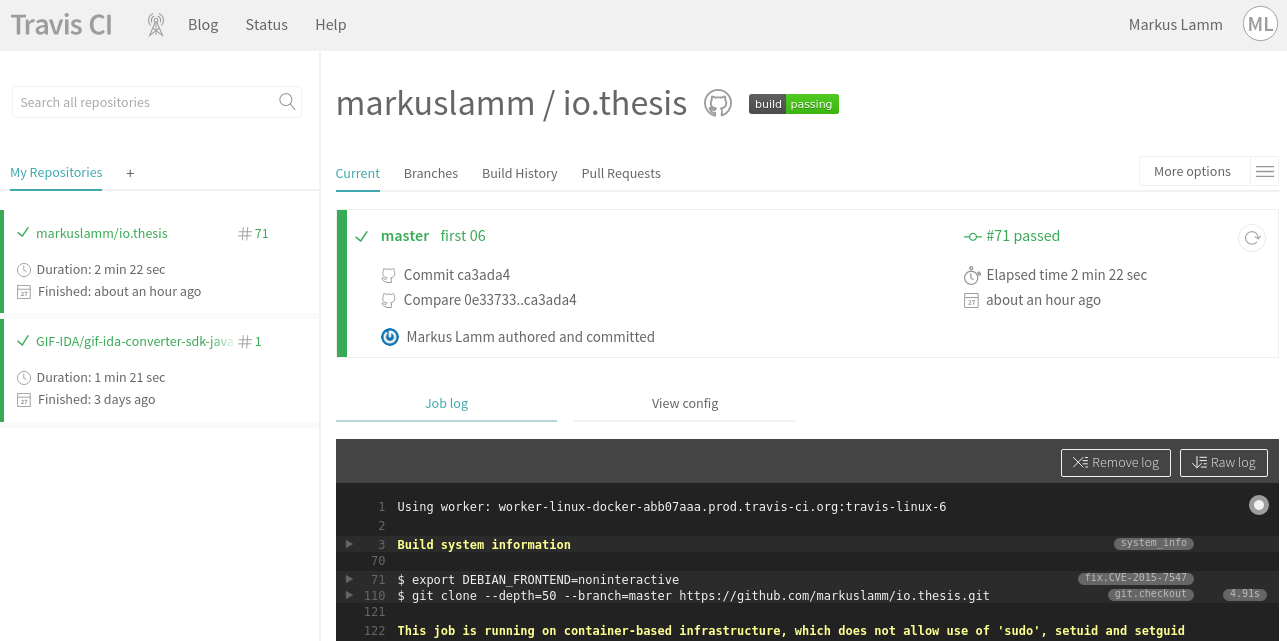
\includegraphics[width=1.0\textwidth]{../images/07-travis.png}
	\caption{Travis CI}
	\label{fig:travis}
\end{figure}

\section{"Collector-Platform" Cluster}
\label{sec:collector-platform-cluster}

According to the proposed architecture in \autoref{ch:architecture}, \textit{"Collector-Platform" Cluster} consists of the
mandatory infrastructure components \textit{Kafka Message-Broker}, \textit{Consul Client-Registry}, \textit{Logstash-Processor} and
\textit{Elasticserach} to fulfill the requirements discussed in \autoref{ch:requirements}. In addition, one instance of
Apache Flink's Job- and TaskManager each will be required, to create a basic Flink cluster acting as data source for the collecting client,
as well as the \textit{Collector-Manager} component for managing the distributed \textit{CollectorClient} instances.

One main challenge of the technical realization of the system solution was to create a cluster of application nodes operating in an
own network distinguishable by their IP addresses. The \textit{"Collector-Platform"} uses Docker to achieve this goal.
Docker provides a "software containerization platform" that allows to wrap applications in a complete filesystem that contains everything
needed to run in form of a container. This container provides an isolated platform for applications to run on Docker host systems
and contains an unix operation system and all required software components required by the application.
Docker uses the resource isolation features of the Linux kernel such as cgroups and kernel namespaces and allow independent containers
to run within a single host instance, avoiding the overhead of starting and maintaining virtual machines.

The applications to be "containerized" will be defined in by a Dockerfile that defines the intructions to build the application container.
The Docker file contains the the behavior of the application when it is started by the \verb|docker-engine|. The following
example shows the definition for the \textit{CollectorManager} component:

\begin{lstlisting}[caption={Dockerfile "CollectorManager"}, captionpos=b, label={lst:dockerfile}]
FROM anapsix/alpine-java
MAINTAINER markus.lamm@googlemail.com
ADD collector-manager-app/target/collector-manager-app.jar /apps/collector-manager-app.jar
ENTRYPOINT ["java","-jar","/apps/collector-manager-app.jar"]
\end{lstlisting}

The resulting container is based on the Docker image \verb|anapsix/alpine-java| which provides an unix operating system and a Java
installation as a base system, the \textit{CollectorManager} will be installed on. In line 3, the \verb|collector-manager-app.jar|
will be copied from the local file system to a virtual path inside the Docker container. The last command in line 4 defines the entry point
for the \verb|docker-engine|, this commmand will be executed on container startup, means the \textit{CollectorManager} jar file will
be executed by the JVM provided by the \verb|anapsix/alpine-java| base image.

Based on the required components discussed above the application needs the following Docker containers:

\begin{itemize}
	\item One Apache Kafka container as message broker and source system for data collection. The Kafka container depends on
	another container for Apache Zookeper as a centralized service for configuration and distributed synchronization and is mandatory
	for the Kafka container to work.
	\item One Consul container as client discovery service
	\item Two Apache Flink containers, one Job- and TaskManager as source systems
	\item One container conatining Logstash, Elasticserach and Kibana
	\item One container for the \textit{CollectorManager} component
\end{itemize}

For the orchestration of the container infrastructure, Docker provides a file format that allows the definion of required containers
and their dependencies in a custom \verb|docker-compose.yml| file. The next section covers main configuration details for the containers
of the \textit{"Collector-Platform"} cluster.

\subsection{Configuration}

The Apache Kafka is a core component of the platform and operates as a buffer between data producing \textit{CollectorClient}s and consuming
\textit{Logstash-Processors}. The following excerpt from the \verb|docker-compose.yml| file defines the container for Kafka:
\begin{lstlisting}[caption={Container definition Kafka}, captionpos=b, label={lst:docker-kafka}]
  kafka:
    container_name: kafka
    image: wurstmeister/kafka
    ports:
      - "9092:9092"
      - "9997:9999"   # jmx
      - "9097:9091"   # collector-client
    environment:
      KAFKA_ZOOKEEPER_CONNECT: zookeeper:2181
      KAFKA_ADVERTISED_HOST_NAME: 192.168.2.100 //THIS NEEDS TO BE ADJUSTED ON LOCAL EVALUATION
      KAFKA_CREATE_TOPICS: "collector-outbound-topic:1:1,flink-outbound-topic:1:1"
      JMX_PORT: 9999
      SPRING_PROFILES_ACTIVE: kafka-broker-jmx
      SPRING_CLOUD_CONSUL_HOST: consul
      SPRING_CLOUD_CONSUL_PORT: 8500
      CLIENT_PORT: 9091
      KAFKA_BROKER_ADDRESS: kafka:9092
    volumes:
      - /var/run/docker.sock:/var/run/docker.sock
    depends_on:
      - zookeeper
      - consul
\end{lstlisting}

This configuration defines the required information for running this container. It defines the required ports and dependencies to other containers,
\verb|zookeeper| and \verb|consul| in this example. Furhermore it creates a set of environment variables, containing
connection infos for zookeeper and the kafka address, that needs to be adjusted to the local IP address. Due to the fact that
this container will also be a source system for the \textit{CollectorClient}s, the JMX port is specified to allow the client to access
the remote JVM of Apache Kafka. Other variables contain information
required by the \textit{CollectorClient} Spring Boot application, that needs to be copied to the Docker description of Apache Kafka.

Another configuration for the definition of the container \textit{CollectorManager}, that defines the required port for the managers user
interface, the dependency to the Consul container as well as environment variables required by the Spring Boot application.

\begin{lstlisting}[caption={CollectorManager container configuration}, captionpos=b, label={lst:docker-manager}]
  collector-manager:
    container_name: collector-manager
    image: io.thesis/collector-manager
    ports:
      - "9090:9090"
    depends_on:
      - consul
    environment:
      SERVER_PORT: 9090
      SPRING_CLOUD_CONSUL_HOST: consul
      SPRING_CLOUD_CONSUL_PORT: 8500
\end{lstlisting}

For the complete configuration of the \textit{"Collector-Platform"} cluster, please refer to Appendix A in \autoref{app:docker-config}

The \verb|docker-compose| file format provides a mechanism to build the \textit{"Collector-Platform"} cluster shown in
\autoref{fig:deployment-diagram}:

\begin{figure}[H]
	\centering
	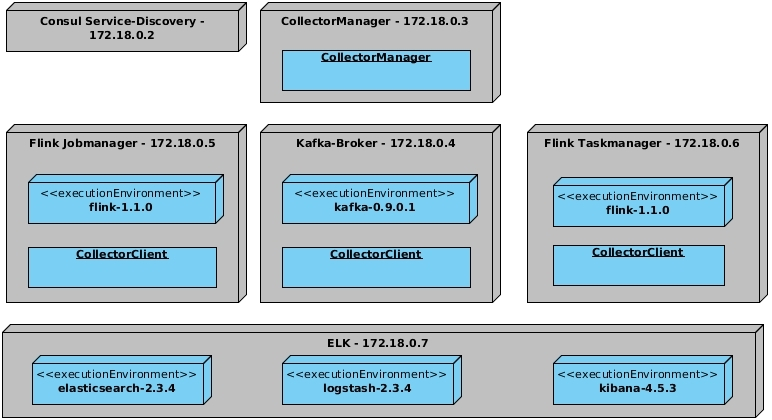
\includegraphics[width=1.0\textwidth]{../uml/deployment-diagram.jpg}
	\caption{Docker Deployment Diagram}
	\label{fig:deployment-diagram}
\end{figure}

To build all required software components and Docker images, and to copy the \verb|collector-client.jar| into the containers of source systems,
the following shell script is used:

\begin{lstlisting}[caption={build-docker-images-sh}, captionpos=b, label={lst:docker-build-images}]
echo "building sources..."
mvn install -DskipTests -DskipITs

echo "cleanup containers..."
docker rm -f $(docker ps -a -q)

echo "building collector-manager-app..."
docker build -t io.thesis/collector-manager collector-manager

echo "building docker-base..."
docker build -t wurstmeister/base infrastructure/docker-base

echo "building docker-zookeeper..."
docker build -t wurstmeister/zookeeper infrastructure/docker-zookeeper

echo "building docker-kafka..."
cp collector-client/collector-client-app/target/collector-client-app.jar infrastructure/docker-kafka/collector-client-app.jar
docker build -t wurstmeister/kafka infrastructure/docker-kafka

echo "building docker-elk..."
docker build -t sebp/elk infrastructure/docker-elk

echo "building docker-flink..."
cp collector-client/collector-client-app/target/collector-client-app.jar infrastructure/docker-flink/collector-client-app.jar
cd infrastructure/docker-flink
./build.sh
\end{lstlisting}

After a successfull building the required software and Docker artefarcts the single command \verb|docker-compose run| starts all
defined containers in the discussed configuration file.

\section{Manual Tests}

The main goal the \textit{Collector-Platform} is to collect system and application data from Apache Flink and Apache Kafka source systems.
Therefore, the system architecture in \autoref{ch:architecture} introduced the \textit{CollectorManager} as the managing component
of distributed \textit{CollectorClient} instances. Hence the \textit{CollectorManager} depends on the Consul Client-Registry,
the Consul container must be up an running. According to the cluster configutation, the Consul container provides a REST endpoint
for listing registered client instances:
\verb|http://localhost:8500|:
\begin{figure}[H]
	\centering
	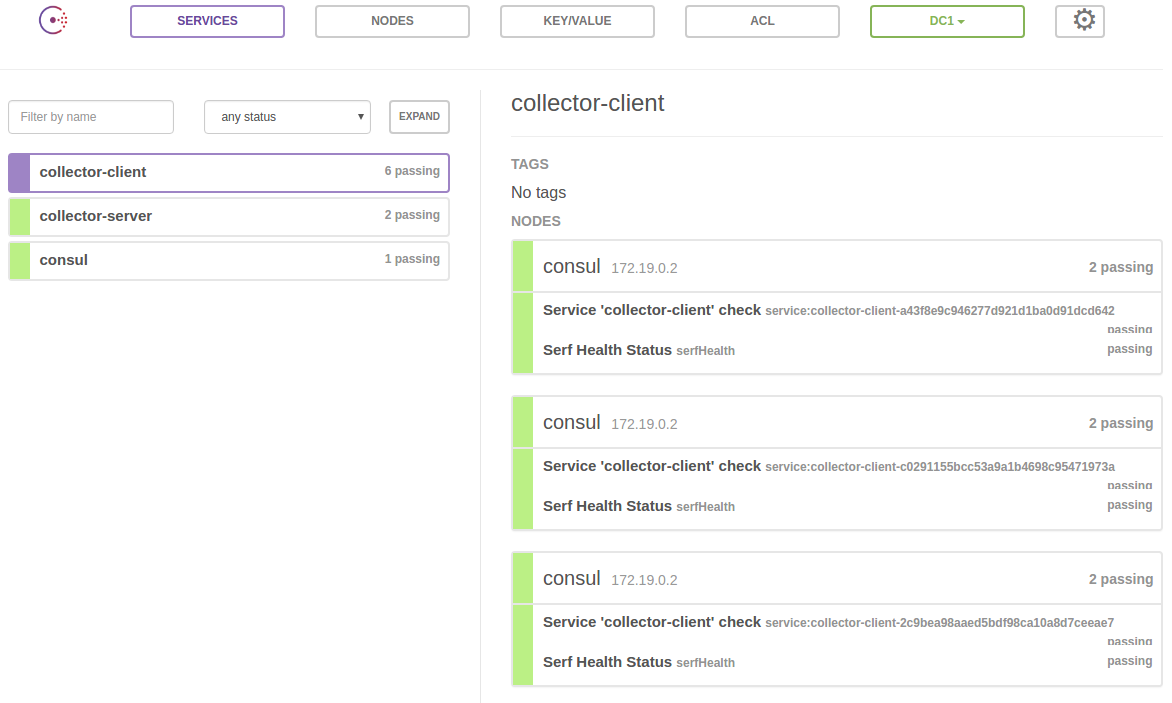
\includegraphics[width=1.0\textwidth]{../images/08-consul.png}
	\caption{Consul web interface}
	\label{fig:consul-web}
\end{figure}

The figure shows three \textit{CollectorClient} instances installed on the \textit{Kafka Message-Broker} as well as the \textit{CollectorClient} instances installed
on the Docker container for Flink's Job- and TaskManager. The presence of the clients in the Consul user interface verifies the
correct functionality of client's self-registrion in the central registry, that is required to list existing clients in
the user interface with the purpose to schedule the data collection process for individual client instances.

The \textit{CollectorManager} is configured to provide the client listing on \verb|http://localhost:9090|:
\begin{figure}[H]
	\centering
	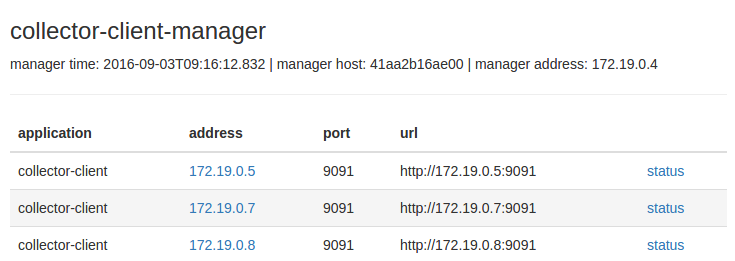
\includegraphics[width=1.0\textwidth]{../images/09-cm-start.png}
	\caption{CollectorManager client listing}
	\label{fig:cm-start}
\end{figure}

In correspondence to \autoref{fig:consul-web}, the \textit{CollectorManager} is able to fetch required client data using the the
\textit{Consul Client-Registry}. This figure shows a very nice feature of Spring Boot, which provides a basic \verb|/health| endpoint for web applications and enables the
\textit{CollectorManager} to link to this endpoint of all \textit{CollectorClient} instances. Because of that, the user interface
of the managing component provides basic monitoring capabilities of registered client instances.

The detailed view of a \textit{CollectorClient} instance provides additinal metadata fetched from the clients \verb|/client/metadata| endpoint.
In addition, the data collection process of the selected client can be started:

\begin{figure}[H]
	\centering
	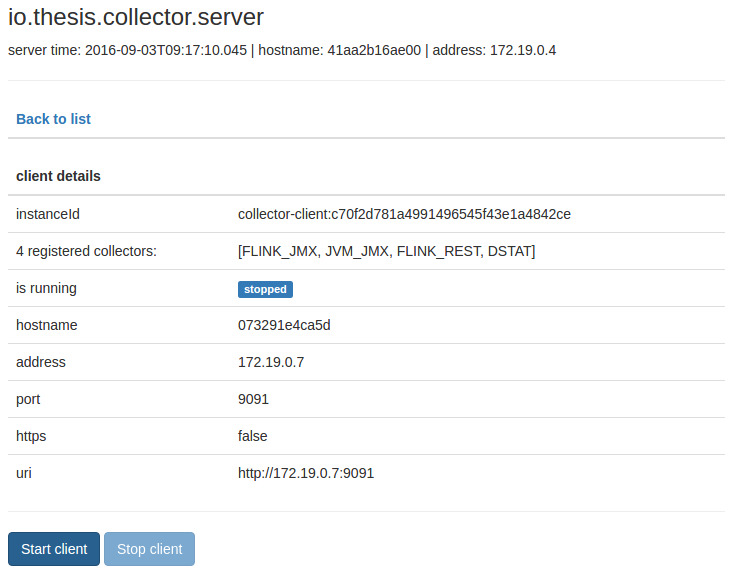
\includegraphics[width=1.0\textwidth]{../images/10-cm-detail.png}
	\caption{CollectorManager client details}
	\label{fig:cm-details}
\end{figure}

The details page for \textit{CollectorClient} shows the unique instance id the client is registred with in the \textit{Consul Client-Registry},
details about the network location and the \textit{Collector} implementations, that are registered in the client as discussed in
\autoref{ch:implementation}. This example shows the \textit{CollectorClient} instance installed on Apache Flink's JobManager,
with registred \textit{Collector} implementations corresponding to the available data sources for Apache Flink introduced in
\autoref{ch:requirements}.

The \verb|"Start client"| button is used to trigger the collection process in the corresponding \textit{CollectorClient} instance and
must start the dataflow of the \textit{Collector-Platform}. Data must be collected, published to the \textit{Kafka Message-Broker} and will
be retrieved by the \textit{Logstash-Processor}, which creates the required indexes in Elasticsearch on the first run.
\begin{verbatim}
[tp1485891705-13] ScheduleController : Received schedule request, action=start
[tp1485891705-13] CollectorClient    : Entering scheduleClient()
[      Thread-14] CollectorClient    : Start collector-client, action='start'
[      Thread-14] CollectorClient    : Entering startCollect()
[      Thread-14] CollectorClient    : Immediately return from startCollect()
[      Thread-15] CollectorClient    : Starting data collection, interval='5000'
[lector-thread-3] CollectorWorker    : Collector worker starts...
[lector-thread-1] CollectorWorker    : Collector worker starts...
[lector-thread-1] DstatCollector     : Entering DSTAT collect()
[lector-thread-1] DstatCollector     : Immediately return from DSTAT collect()
[lector-thread-1] CollectorWorker    : Collector worker finished
[lector-thread-1] CollectorWorker    : Collector worker starts...
[lector-thread-3] CollectorWorker    : Collector worker finished
[lector-thread-3] CollectorWorker    : Collector worker starts...
...
[      Thread-18] KafkaOutboundWriter: Trying to send data to Kafka
...
[ad | producer-1] KafkaOutboundWriter : Successfully send to Kafka, key=flink_rest
[ad | producer-1] KafkaOutboundWriter : Successfully send to Kafka, key=jvm_jmx
[ad | producer-1] KafkaOutboundWriter : Successfully send to Kafka, key=jvm_jmx
[ad | producer-1] KafkaOutboundWriter : Successfully send to Kafka, key=flink_rest
[ad | producer-1] KafkaOutboundWriter : Successfully send to Kafka, key=flink_jmx
...
[cluster.metadata] [flink_rest_collector_raw_index]
[cluster.metadata] [jvm_jmx_collector_raw_index]
[cluster.metadata] [flink_jmx_collector_raw_index]
...
\end{verbatim}

The logs produced by individual containers will be aggregated in the terminal the cluster is started in and, the example shows the
abbreviated output after starting data collection by pressing the "Start client" button, which results the the alert based on the response data:

\begin{figure}[H]
	\centering
	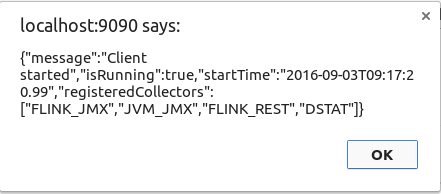
\includegraphics[width=0.5\textwidth]{../images/11-alert.png}
	\caption{Client response}
	\label{fig:alert}
\end{figure}

To list existing indexes in Elasticsearch to verify that required indexex are created correctly, the search engine provides a
REST resource for this purpose, the request for \verb|http://localhost:9200/_cat/indices?v| produces the following output and verifies
that the indexes for registered \textit{Collector} implementations are created.
\begin{figure}[H]
	\centering
	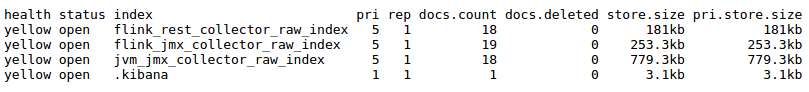
\includegraphics[width=1.0\textwidth]{../images/12-indexes.png}
	\caption{Elasticsearch indexes}
	\label{fig:indexes}
\end{figure}

The attentive reader will notice that there is no index created for the Dstat collector source implementation! This is caused, because
it was not possible to read the output of the Dstat process if the process is started in a Docker container, the result was always empty
and the problem couldn't be fixed in time! \autoref{app:dstat-result} contains the result of the \verb|DstatCollector| produced
on the local machine in a non-Docker environment.


At this point, the architectural requirements of a central registry for \textit{CollectorClient} instances, the data collection on the
Apache Flink source system, the transport of data to the \textit{Logstash-Processor} via \textit{Kafka Message-Broker} and creating required
indexes for the storage of collected data can be verified.

To access collected data, Elasticsearch provides rich REST interface for quering the data stored in a given index, but the the ELK-Stack
comes with Kibana, a visualization tool for time-series based data. On the example of the index created for storing data of the
\verb|FlinkRestCollector|, the following figure shows an overview of existing data in this index:
\begin{figure}[H]
	\centering
	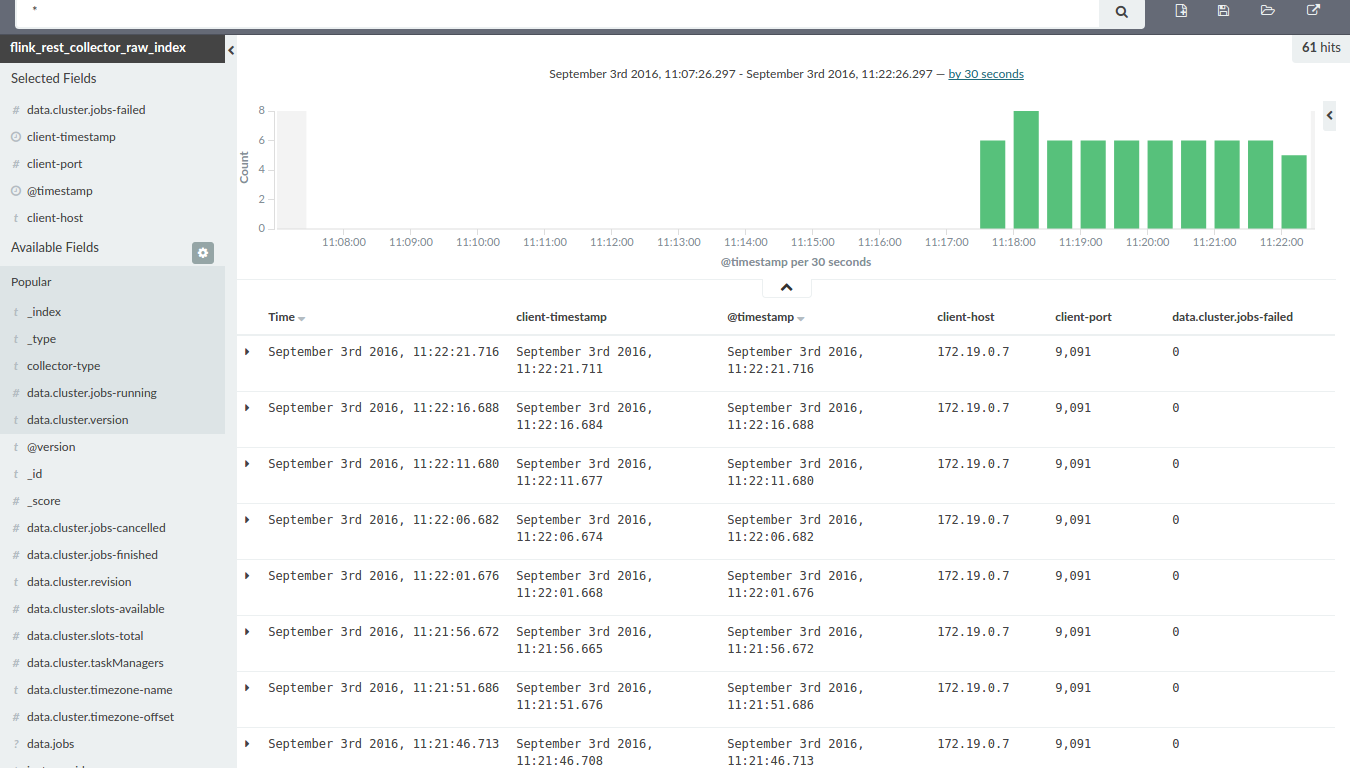
\includegraphics[width=1.0\textwidth]{../images/13-kibana.png}
	\caption{FlinkRestCollector data overview}
	\label{fig:kibana}
\end{figure}

As shown above, the collected is available, it contains the client timestamp, the timestamp the data received in Elasticsearch, clients
identification data in form of IP address and port as well as the data produced by the \textit{Collector} implementation.
This is the end of the data pipeline in the \textit{Collector-Platform}. The same process will be repeated in the configurable interval
of 5 seconds per default until it will be stopped performing the appropriate REST request on the \textit{CollectorClient}.

The section above refers to the usage of the Apache Flink JobManager source system. The same examination can be made concerning
the listed clients in \autoref{fig:cm-start} located on the TaskManager container and Kafka Message-Broker respectively.

\section{Consumer Integration}

To demonstrate the flexibility of the proposed architecture for the integration of potential data consumers, the prototype application
provides an additional Maven module named \verb|collector-data-processor|, a stream processing component based on Apache Flink.

\begin{lstlisting}[caption={Apache Flink raw data stream processor}, captionpos=b, label={lst:flink-processor},language=Java]
...
private static final String INBOUND_TOPIC = "collector-outbound-topic";
private static final String OUTBOUND_TOPIC = "flink-outbound-topic";

final DataStream<CollectorResult> mappedStream =
    env.addSource(new FlinkKafkaConsumer09<>(INBOUND_TOPIC, new SimpleStringSchema(), properties))
        .flatMap((rawJsonInput, out) -> {
            final CollectorResult collectorResult = JsonUtils.readObject(CollectorResult.class, rawJsonInput);
            out.collect(collectorResult);
        });  ## (1)

final DataStream<CollectorResult> collectorFlinkJmxStream = mappedStream.filter(collectorResult ->
    collectorResult.getCollectorType().equals("flink_jmx")); ## (2)

final DataStream<String> resultStream = collectorFlinkJmxStream.map(flinkJmxResult -> {
    final Map<String, Object> dataMap = new LinkedHashMap<>(); ## (3,4)
    dataMap.put("client-timestamp", extractOrUnknown(flinkJmxResult.getClientTimestamp()));
    dataMap.put("client-host", extractOrUnknown(flinkJmxResult.getClientHost()));
    dataMap.put("client-port", extractOrUnknown(flinkJmxResult.getClientPort()));
    dataMap.put("client-instance-id", extractOrUnknown(flinkJmxResult.getInstanceId()));
    final Map<String, Object> jvmMap = Optional.ofNullable(flinkJmxResult.getData())
        .map(CollectorDataProcessor::extractJvmData)
        .orElse(new LinkedHashMap<>());
    dataMap.putAll(jvmMap);
    return JsonUtils.toJson(dataMap);
    });
    resultStream.addSink(new FlinkKafkaProducer09<>(KAFKA_HOST, OUTBOUND_TOPIC, new SimpleStringSchema())); ## (5)
    env.execute();
\end{lstlisting}

This Apache Flink component receives the raw data of distributed \textit{CollectorClients} by subscribing to the \verb|collector-outbound-topic|,
which is the same the clients publish the data to. The data comes in its JSON representation and will be converted into a \verb|CollectorResult|
object (1). The next step in the data flow is the filtering of incoming messages, the stream processor is just interested in data
produced by the \textit{Collector} implementation of the type \verb|flink_jmx| (2). This data collected by the  \verb|FlinkJmxCollector| class contains
inter alia basic infos concerning cpu load and time of the source system. The raw data that matches this criterion will be parsed and
the client identification data as well as the values for cpu load and time will be extracted (3,4). The last step is to publish the
extracted data into the \verb|flink-outbound-topic|, which the \textit{Logstash-Processor} is a subscriber of, hence the "flattened"
cpu metrics will be written in a corresponding \verb|flink_job_index| in Elasticsearch. The processed data can now be discovered using approriate Kibana visualization.

\begin{figure}[H]
	\centering
	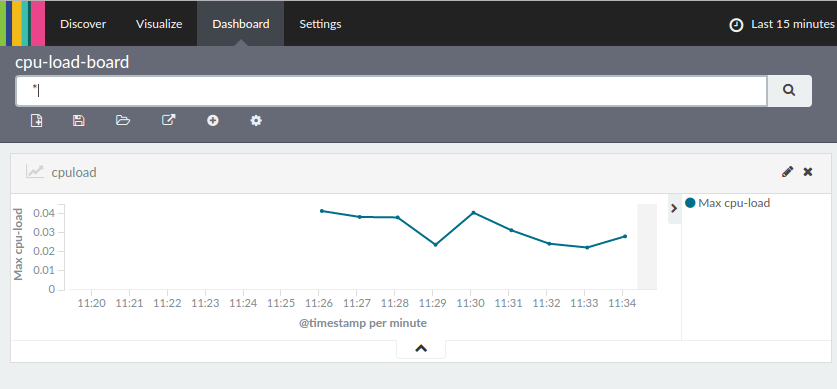
\includegraphics[width=1.0\textwidth]{../images/14-kibana-cpu.png}
	\caption{Kibana cpu load visualization}
	\label{fig:kibana-cpu}
\end{figure}

\section{Discussion}

Based on the evaluation of the \textit{"Collector-Platform} above, following statements can be made regarding to the functional and
non-funtional requirements defined in \autoref{sec:fr} and \autoref{sec:nfr}:

The proposed system solution meets all functional requirements. The \textit{CollectorClient} allows the data collection on
Apache Flink and Apache Kafka source systems wherein the client uses a configurable and internal registration of \textit{Collector} implementations.
The clients create a stream of collected data, that represents the system and application state of the underlying source systems at
a given point of time. Resulting data will be stored in its raw JSON structure in appropriate Elasticsearch indexes where it is available
for analyzing, querying and visualization.

The non-functional requirements contain the criterion \textit{Performance} which includes the impact on source systems as well as the elapsed time
from data collection until it becomes becomes available for potential consumers, a period of two seconds was defined. \autoref{fig:kibana}
shows the data of the \verb|FlinkRestCollector|. The example shows that based on the value for \verb|clientTimestamp|, the value the data has left the client,
and \verb|@timestamp|, the time the data arrived the \textit{Logstash-Processor}, all messages arrive within a period of 10 ms maximum,
which definitely meets the criterion and and demonstrates the "real-time" capabilities of the chosen system architecture.

A negative impact on source systems wasn't examined on the local cluster, but should be considered for "real" applications. The implementation
of as much "non-blocking" code as possible was introduced to in \autoref{ch:implementation} and forces a more effective utilization
of existing resources by implementing a asynchronous interaction using the multithreading environment.

The platform also meets the criterion of \textit{Extensibility}. The pipelined architecture can be easy adapted for other source systems
like Apache Spark, the approach to decouple the \textit{CollectorClient} implementation from concrete \textit{Collector} implementations
allows a lightweight registration for other collectors. On architectural level, the system becomes very flexible by using a \textit{Kafka Message-Broker}
as a data buffer between data consumers and producers. As shown in \autoref{lst:flink-processor}, potential consumers can be plugged in easily
by subscribing to the topics they are interested in. Additionally, the \textit{"Collector-Platform"} doesn't depend on Elasticsearch
for storing raw and/or processed data. As long a the storage system allows to persist streaming data from Apache Kafka, the system can be changed.
For example, a Cassandra cluster would be possible because integration for Kafka exist. In addition, this approach makes the architecture portable
and simple, produces and consumers doesn't require any special operation for exchanging data.

The \textit{"Collector-Platform"} is very scalable, the streaming architecture doesn't care whether to collect from a single system
or multiple nodes in a cluster. More data sources can be integrated into the cluster introduced in \autoref{fig:deployment-diagram} easily
by providing more source containers in the configuration of the cluster.

\section{Summary}

The last chapter introduced the concept of automated unit and integration tests to ensure the functinality of produced application code and their
interaction with dependent components. The separation of unit tests that will be executed in the Maven \verb|test| phase and integration
tests that require a running infrastructure for collecting data from led to the introduction of the \textit{"Collector-Platform} Cluster,
the overall, Docker based system containing the required components defined in \autoref{ch:architecture}.

Based on the cluster setup, the main process of data collection, transport and storage had been demonstrated and evaluated on the example of
an Apache Flink source system, which was also used to demonstrate the integration capabilities of data consumers, by using a simple
stream processing application for extracting cpu metrics data and their visualization in Kibana.

The platform for collecting data of streaming applications became a streaming platform itself! The streaming approach using Kafka,
Logstash and Elasticsearch provides a very flexible and scalable solution that mets all functional and non-functional requirements defined in \autoref{ch:requirements}.